\documentclass[a3]{sciposter}
\usepackage{graphicx}
\usepackage{color}
\usepackage{multicol}
\usepackage{url}
\usepackage{ragged2e}
\usepackage{watermark}

\newcommand{\figfigure}[2]{%
  \includegraphics[width=#1]{#2}
}

\setlength{\columnsep}{10pt}

\title{\vspace*{-0.7cm}
  The \textcolor{red}{igraph} library for network analysis}
\author{\vspace*{-0.5cm}
  \normalsize G\'abor Cs\'ardi$^{1,2}$ and 
  Tam\'as Nepusz$^{1,3}$}
\institute{\small\mbox{}$^1$Department of Biophysics, 
  Research Institute for Particle and Nuclear Physics \\
  of the Hungarian Academy of Sciences,
  Budapest, Hungary. \\
  \mbox{}$^2$Center for Complex Systems Studies, Kalamazoo College,
  Kalamazoo, MI, USA. \\
  \mbox{}$^3$Dept. of Measurement and Information Systems, Budapest
  University of Technology and Economics, Budapest, Hungary.
}
% \email{\small csardi@rmki.kfki.hu \& ntamas@rmki.kfki.hu}
\leftlogo{RMKI-BME}
\rightlogo{CCSS}

\setlength{\parskip}{5pt}

\begin{document}

\watermark{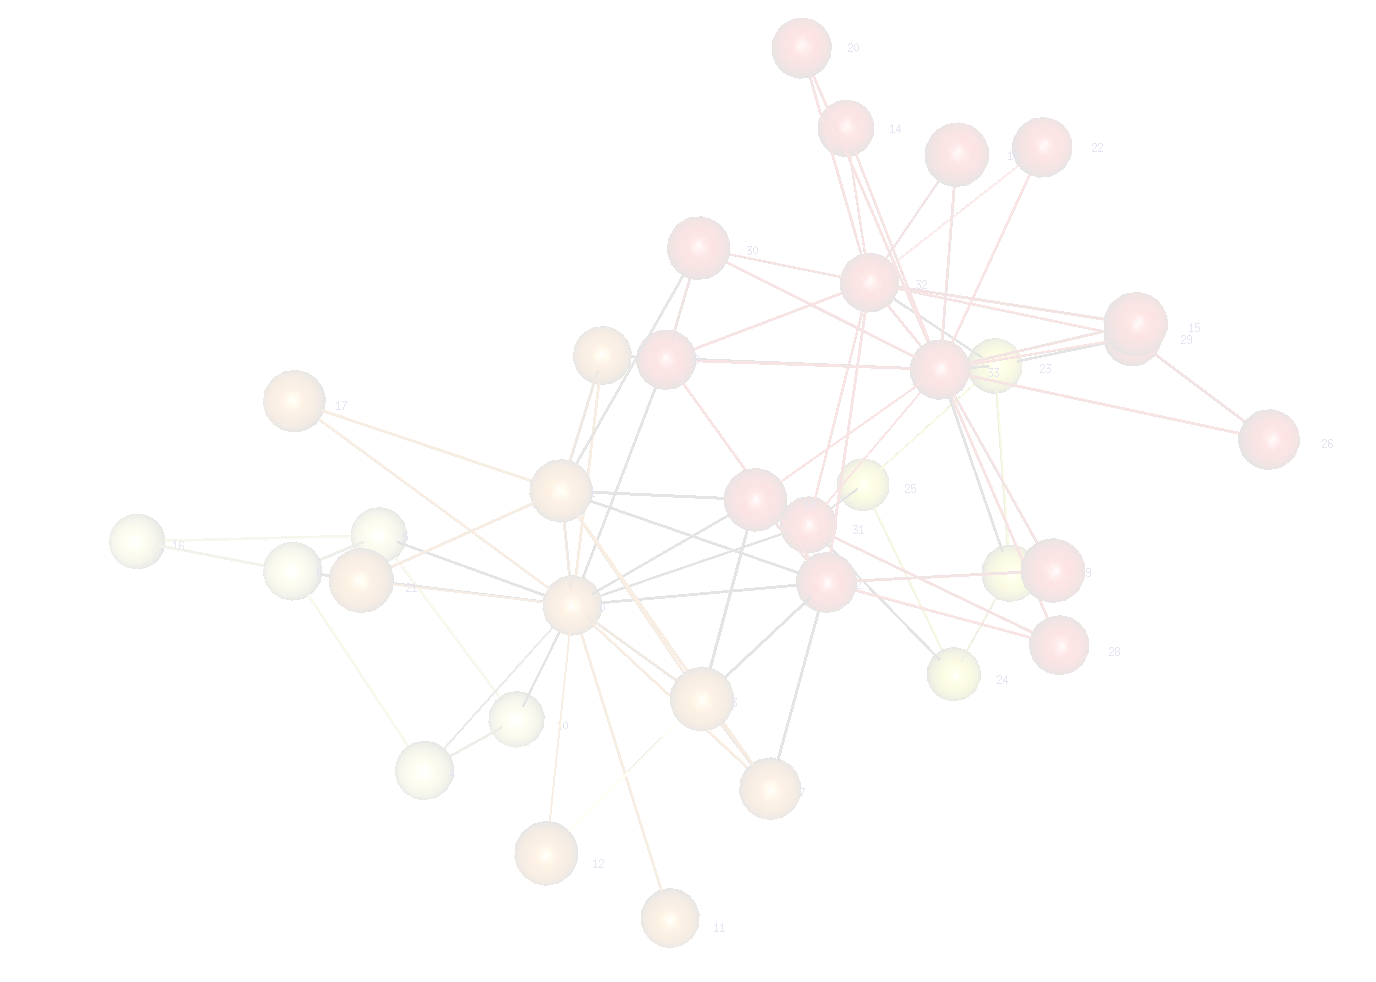
\includegraphics[angle=-90,width=\textwidth]{karate3d}}

\vspace*{-0.8cm}
{\small
\maketitle
}

\enlargethispage{1cm}

\vspace*{-0.7cm}
\vfill
\hrule
\vfill
\vspace*{-0.3cm}
\begin{multicols}{3}

\RaggedRight

%%%%%%%%%%%%%%%%%%%%%%%%%%%%%%%%%%%%%%%%%%%%%%%%%%%%%%%%%%%%%%%%%%
%% \section{Goals}
%% \begin{itemize}
%% \item Ability to handle large graphs efficiently.
%% \item Embeddable into higher level environments like GNU R or Python.
%% \item Ability to be used for quick prototyping.
%% \end{itemize}

%%%%%%%%%%%%%%%%%%%%%%%%%%%%%%%%%%%%%%%%%%%%%%%%%%%%%%%%%%%%%%%%%%
\section{Features}

\begin{itemize}
\item Efficient implementation. The current state of the art
  algorithms are implemented (if not that is considered as a bug).
\item Portable C (and some C++) code, works on most platforms:
  Linux flavours, MS Windows variations, Mac OSX, Solaris, etc.
\item Wide variety of graph algorithms: random and regular graph
  structures, centrality measures, shortest paths, 2D and 3D graph
  layouts, graph motifs, cliques, network flows and cuts, community
  structure detection, etc.
\item Interfaces from GNU R and Python, other interfaces can be added
  without too much hassle.
\item Interactive and non-interactive, 2D and 3D
  visualization from R and Python.
\item Graph, vertex and edge attributes, like edge weights, vertex
  colors and other parameters for plotting.
\item Various import and export file formats: GraphML, Pajek, simple
  edge list, etc.
\item Well documented.
\item Open source and completely free for non-commercial and
  commercial use.
\end{itemize}

%%%%%%%%%%%%%%%%%%%%%%%%%%%%%%%%%%%%%%%%%%%%%%%%%%%%%%%%%%%%%%%%%%
\section{Where to get it?}
\centerline{\bf \url{http://igraph.sf.net}}

You can also find here the source code producing these screenshots.

%%%%%%%%%%%%%%%%%%%%%%%%%%%%%%%%%%%%%%%%%%%%%%%%%%%%%%%%%%%%%%%%%%
\vfill\columnbreak
\section{Architecture}

Simple and flexible layered architecture.
Modules interact via well-defined interfaces and 
can be replaced individually without breaking other parts.

\begin{center}
\figfigure{\columnwidth}{arch}
\end{center}

%%%%%%%%%%%%%%%%%%%%%%%%%%%%%%%%%%%%%%%%%%%%%%%%%%%%%%%%%%%%%%%%%%
%% \section{Examples and screenshots}

\hrule
\vfill
\url{{csardi,ntamas}@rmki.kfki.hu}
\end{multicols}

\vfill
\hrule
\vfill

\centerline{\includegraphics[width=\textwidth]{screenshots}}
\vspace*{-0.3cm}
\centerline{\small Information Visualization Software Infrastructures Workshop, Z\"urich, 2007}
\vfill

\end{document}

